%% Slides for ".NET Programming" by Chunyu Wang <chunyu@hit.edu.cn> %%

\section{.NET 开发工具}

\begin{frame}[fragile]
\frametitle{传统的 Windows 开发}

\CJKindent 创建并显示一个窗口:

\lstset{language=C}
\begin{lstlisting}
HWND hwndMain = CreateWindowEx( 0,
  "MainWinClass", "Main Window",
  WS_OVERLAPPEDWINDOW | WS_HSCROLL |
  CW_USEDEFAULT, CW_USEDEFAULT,
  CW_USEDEFAULT, CW_USEDEFAULT,
  (HWND) NULL, (HWND) NULL,
  hInstance, NULL);

ShowWindow(hwndMain, SW_SHOWDEFAULT);

UpdateWindow(hwndMain);
\end{lstlisting}

\end{frame}

\begin{frame}[fragile]
\frametitle{.NET 中的开发}
创建并显示一个窗口:

VB.NET
\lstset{defaultdialect=[Visual]Basic,language=Basic}
\begin{lstlisting}
Dim form1 as New Form()
form1.Text = "New Window"
form1.Show()
\end{lstlisting}

C\#
\lstset{language=CSharp}
\begin{lstlisting}
Form form1 = new Form();
form1.Text = "Main Window";
form1.Show();
\end{lstlisting}
\end{frame}

\begin{frame}
\frametitle{.NET 编程语言}
\framesubtitle{Microsoft 提供编程语言}

\begin{itemize}
  \CJKindent
\item Visual C\# .NET  \par
  \smallskip \small .NET 平台首推的开发语言
\item Visual Basic .NET \par
  \smallskip \small 方便 VB 程序员进行 .NET 开发
\item Visual C++ .NET (Managed C++) \par
  \smallskip \small 同时利用 C++ 和 .NET 平台(类库)
\item Visual J\# .NET (Java) \par
  \smallskip \small 方便 Java 程序员,移植现有 Java 项目到 .NET 平台
\item JScript .NET \par
  \smallskip \small 使用 JScript 利用 .NET 平台(类库)
\end{itemize}
\end{frame}

\begin{frame}
\frametitle{.NET 编程语言}
\framesubtitle{其他可以在 .NET 平台编译的语言 }
\begin{columns}[t]
  \column{.28\textwidth}
  \begin{itemize}
    \setlength{\itemsep}{8pt plus 1pt}
  \item Fortran
  \item Python
  \item Perl
  \item Scheme
  \item Haskell
  \item Smalltalk
  \end{itemize}
  \column{.28\textwidth}
  \begin{itemize}
    \setlength{\itemsep}{8pt plus 1pt}
  \item F\#
  \item COBOL
  \item Mercury
  \item Mondrian
  \item Oberon
  \item Eiffel\#
  \end{itemize}
  \column{.44\textwidth}
  \begin{itemize}
    \setlength{\itemsep}{8pt plus 1pt}
  \item Component Pascal
  \item RPG
  \item Delta Forth
  \item Standard ML
  \item TMT Pascal
  \item $\ldots$
  \end{itemize}
\end{columns}
\end{frame}


\begin{frame}
\frametitle{.NET 开发工具}

\begin{exampleblock}{\textit{Microsoft .NET Framework Redistributable}}
  \CJKindent .NET 框架可再发行组件包,包括 .NET Framework 应用程序运行所需的库及相关文件。
\end{exampleblock}
\pause
\begin{exampleblock}{\textit{Software Development Kit (SDK)}}
  \CJKindent .NET 框架开发工具包,包括了编写、生成、测试和部署 .NET Framework 应用程序所需的工具、文档和示例。
\end{exampleblock}
\pause
\begin{block}{\textit{Visual Studio .NET}}
  \CJKindent Visual Studio 是一套完整的开发工具集,用于生成 ASP.NET Web 应用程序、XML Web Services、
  桌面应用程序和移动应用程序。Visual Basic、Visual C++、Visual C\# 和 Visual J\# 全都使用相同的集成开发
  环境。
\end{block}

\end{frame}

\begin{frame}[t]
\frametitle{SDK 中的工具 --- \textit{csc}}
\begin{exampleblock}{C\# 编译器 csc.exe}
  \begin{tabular}{l|l}
    \hline
    \multicolumn{1}{c|}{Option}      & \multicolumn{1}{c}{Description}                  \\\hline
    \texttt{/help}                   & 列出所有命令行选项                               \\
    \texttt{/define:\textsl{symbol}} & 定义编译预处理符号                               \\
    \texttt{/doc:\textsl{name}}      & 从源码 XML 注释中生成 XML 文档                 \\
    \texttt{/out:\textsl{name}}      & 输出文件名                                       \\
    \texttt{/target:\textsl{target}} & 输出文件格式 {\small exe/winexe/library/module} \\
    \hline
  \end{tabular}
\end{exampleblock}
\setbeamertemplate{blocks}[rounded][shadow=true]
\pause

\begin{alertblock}{}
  \texttt{csc /target:exe     /out:Hello.exe MyHello.cs}\\
  \texttt{csc /target:library /out:Hello.dll MyHello.cs}
\end{alertblock}

\begin{alertblock}{}
  \texttt{csc /target:module A.cs}\\
  \texttt{csc /out:Final.dll /addmodule:A.netmodule \wraphere \hskip.12\textwidth /target:library B.cs}
\end{alertblock}
\end{frame}

\begin{frame}[fragile,t]
\frametitle{SDK 中的工具 --- \textit{ildasm}}
\begin{exampleblock}{MSIL 的反编译工具 ildasm.exe}
  \uncover<1-| handout:1>{  \texttt{csc /target:exe     /out:Hello.exe MyHello.cs}\\}
  \uncover<2-| handout:1>{  \texttt{ildasm Hello.exe}\\
  }
\end{exampleblock}
\begin{onlyenv}<1| handout:0>
\begin{lstlisting}
using System;
class Hello
{
  public static void Main ()
  {
    Console.WriteLine("Hello World!");
  }
}
\end{lstlisting}
\end{onlyenv}

\includegraphics[scale=.5]<2| handout:1>{ildasm1}%
\rlap{\includegraphics[scale=.5]<3| handout:0>{ildasm2}}%

\end{frame}

\begin{frame}
\frametitle{SDK 中的工具 --- \textit{others}}

\begin{itemize}
    \setlength{\itemsep}{6pt plus 1pt}
\item vbc.exe --- VB.NET 编译工具
\item cl.exe  --- C++ 编译工具
\item al.exe  --- 程序集生成工具
\item ilasm.exe --- MSIL 的编译工具
\item dumpbin.exe --- PE 文件查看工具
\item ngen.exe --- 本地镜像生成工具
\item xsd.exe --- XML 模式定义工具
\item sn.exe --- 增强名工具
\end{itemize}
\end{frame}

\begin{frame}
\frametitle{Microsoft Visual Studio 2008}
\begin{itemize}
    \setlength{\itemsep}{8pt plus 1pt}
\item 多种开发语言共存,使用同样的开发方式
\item 与 MSDN 共享同一个 IDE
\item 动态帮助,代码自动生成
\item 集成 Web 浏览器
\item 各种设计的图形视图
\end{itemize}
\end{frame}

\begin{frame}
\frametitle{Microsoft Visual Studio 2008}
\begin{block}{解决方案}
  \CJKindent \small 解决方案管理 Visual Studio 配置、生成和部署相关项目集的方式。Visual Studio 解决方
  案可以只包含一个项目,也可以包含由开发小组联合生成的多个项目。复杂的应用程序可能需要多个解决方案。
\end{block}
\begin{figure}
  \centering
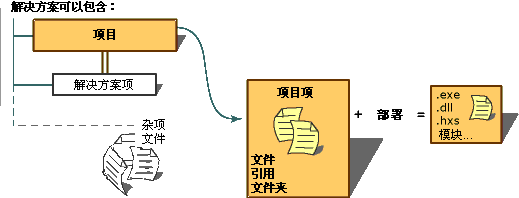
\includegraphics[width=10cm]{vstudio-proj}
\end{figure}
\end{frame}

\begin{frame}
\frametitle{Microsoft Visual Studio 2008}
新建项目:
\begin{columns}
\column{.5\textwidth}
  \begin{itemize}
  \item Console Application
  \item Windows Application
  \end{itemize}
\column{.5\textwidth}
  \begin{itemize}
  \item Class Library
  \item Windows Control Library
  \end{itemize}
\end{columns}
\begin{figure}
  \centering
  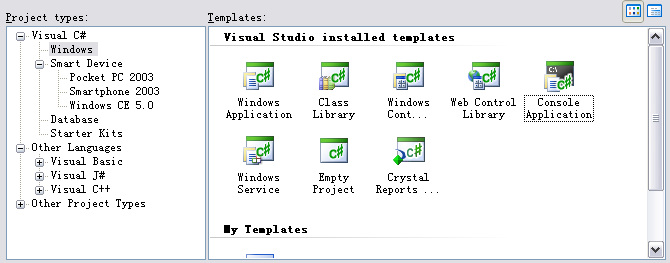
\includegraphics[width=10cm]{vstudio-newp}
\end{figure}
\end{frame}

\begin{frame}
\frametitle{Microsoft Visual Studio 2008}
\begin{columns}
\column{.5\textwidth}
调试的基本功能
  \begin{itemize}
  \item 开始运行 F5/Ctrl-F5
  \item 单步跟踪 F11/F10
  \item 设置断点 Ctrl-B
  \item 查看表达式值 Ctrl-D Q
  \end{itemize}
常用的工具视图
  \begin{itemize}
  \item Solution Explore (Ctrl-W S)
  \item Property Window (Ctrl-W P)
  \item ToolBox (Ctrl-W X)
  \item Class View (Ctrl-W C)
  \end{itemize}
\column{.5\textwidth}
\begin{figure}
  \centering
  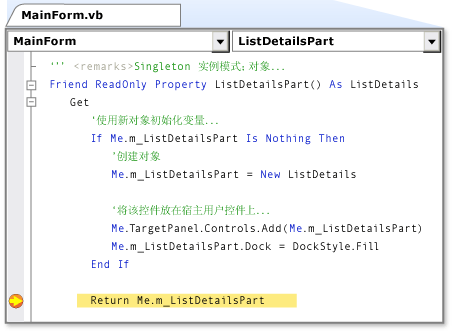
\includegraphics[width=5cm]{vstudio-debg}
\end{figure}
\end{columns}
\end{frame}

\begin{frame}
\frametitle{编程语言排行榜(TIOBE)}
\begin{itemize}
\item 2011--08: F\# enters the top 20 for the first time
\item {\scriptsize http://www.tiobe.com/index.php/content/paperinfo/tpci/index.html}
\end{itemize}
\centering
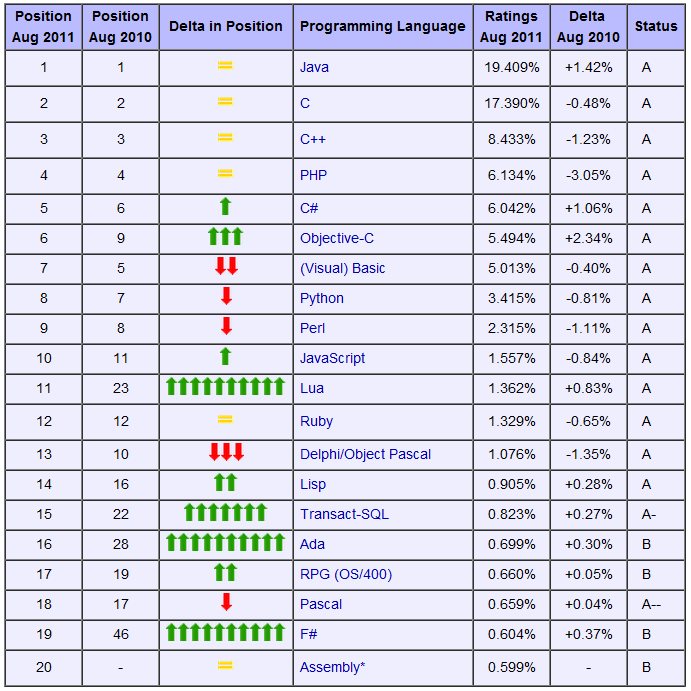
\includegraphics[width=5cm]{tiobe-201108}
\end{frame}

\begin{frame}
\frametitle{编程语言排行榜(TIOBE)}
\begin{itemize}
\item 2011--09: C\# 超过 PHP
\end{itemize}
\centering
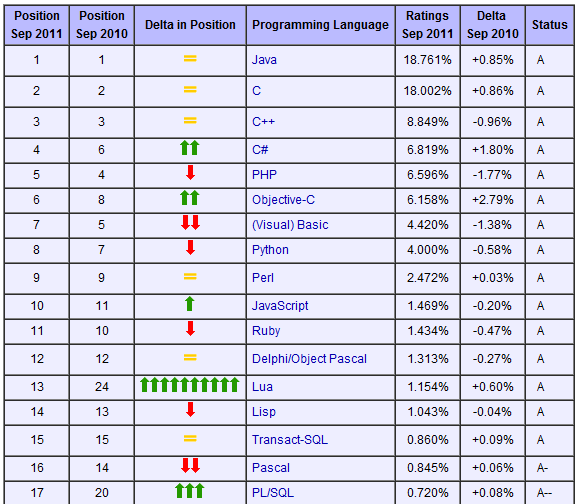
\includegraphics[width=5cm]{tiobe-201109}
\end{frame}

\begin{frame}
\frametitle{编程语言排行榜(TIOBE)}
\begin{itemize}
\item 5, 10, 15 年 top10 排名
\end{itemize}
\centering
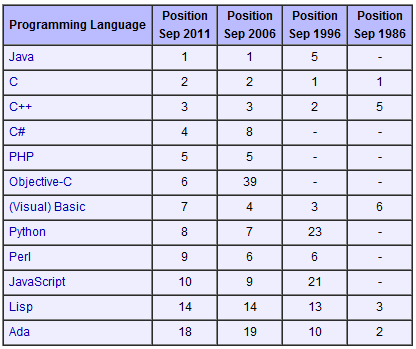
\includegraphics[width=5cm]{tiobe-long}
\end{frame}


% Local Variables:
% mode: LaTeX
% TeX-master: "part-01.tex"
% TeX-header-end: "% End-of-Header$"
% TeX-trailer-start: "% Start-of-Trailer$"
% fill-column: 100
% coding: utf-8
% End:
